% ════════════════════════════════════════════
% 结论与建议（07.模型评价.tex）
% ════════════════════════════════════════════
\section{结论与建议}

\subsection{主要结论}

本报告围绕品牌主页帖子曝光量的影响因素，完成了从数据理解、清洗编码、回归诊断到效应测算的完整分析。图\ref{fig:summary}把核心结论集中呈现：付费投放平均带来约四成曝光提升，内容类型差异明显，内容主题整体显著且付费效应随主题变化，发帖决策解释的方差约为规模与时间的两倍。

\begin{figure}[ht]
  \centering
  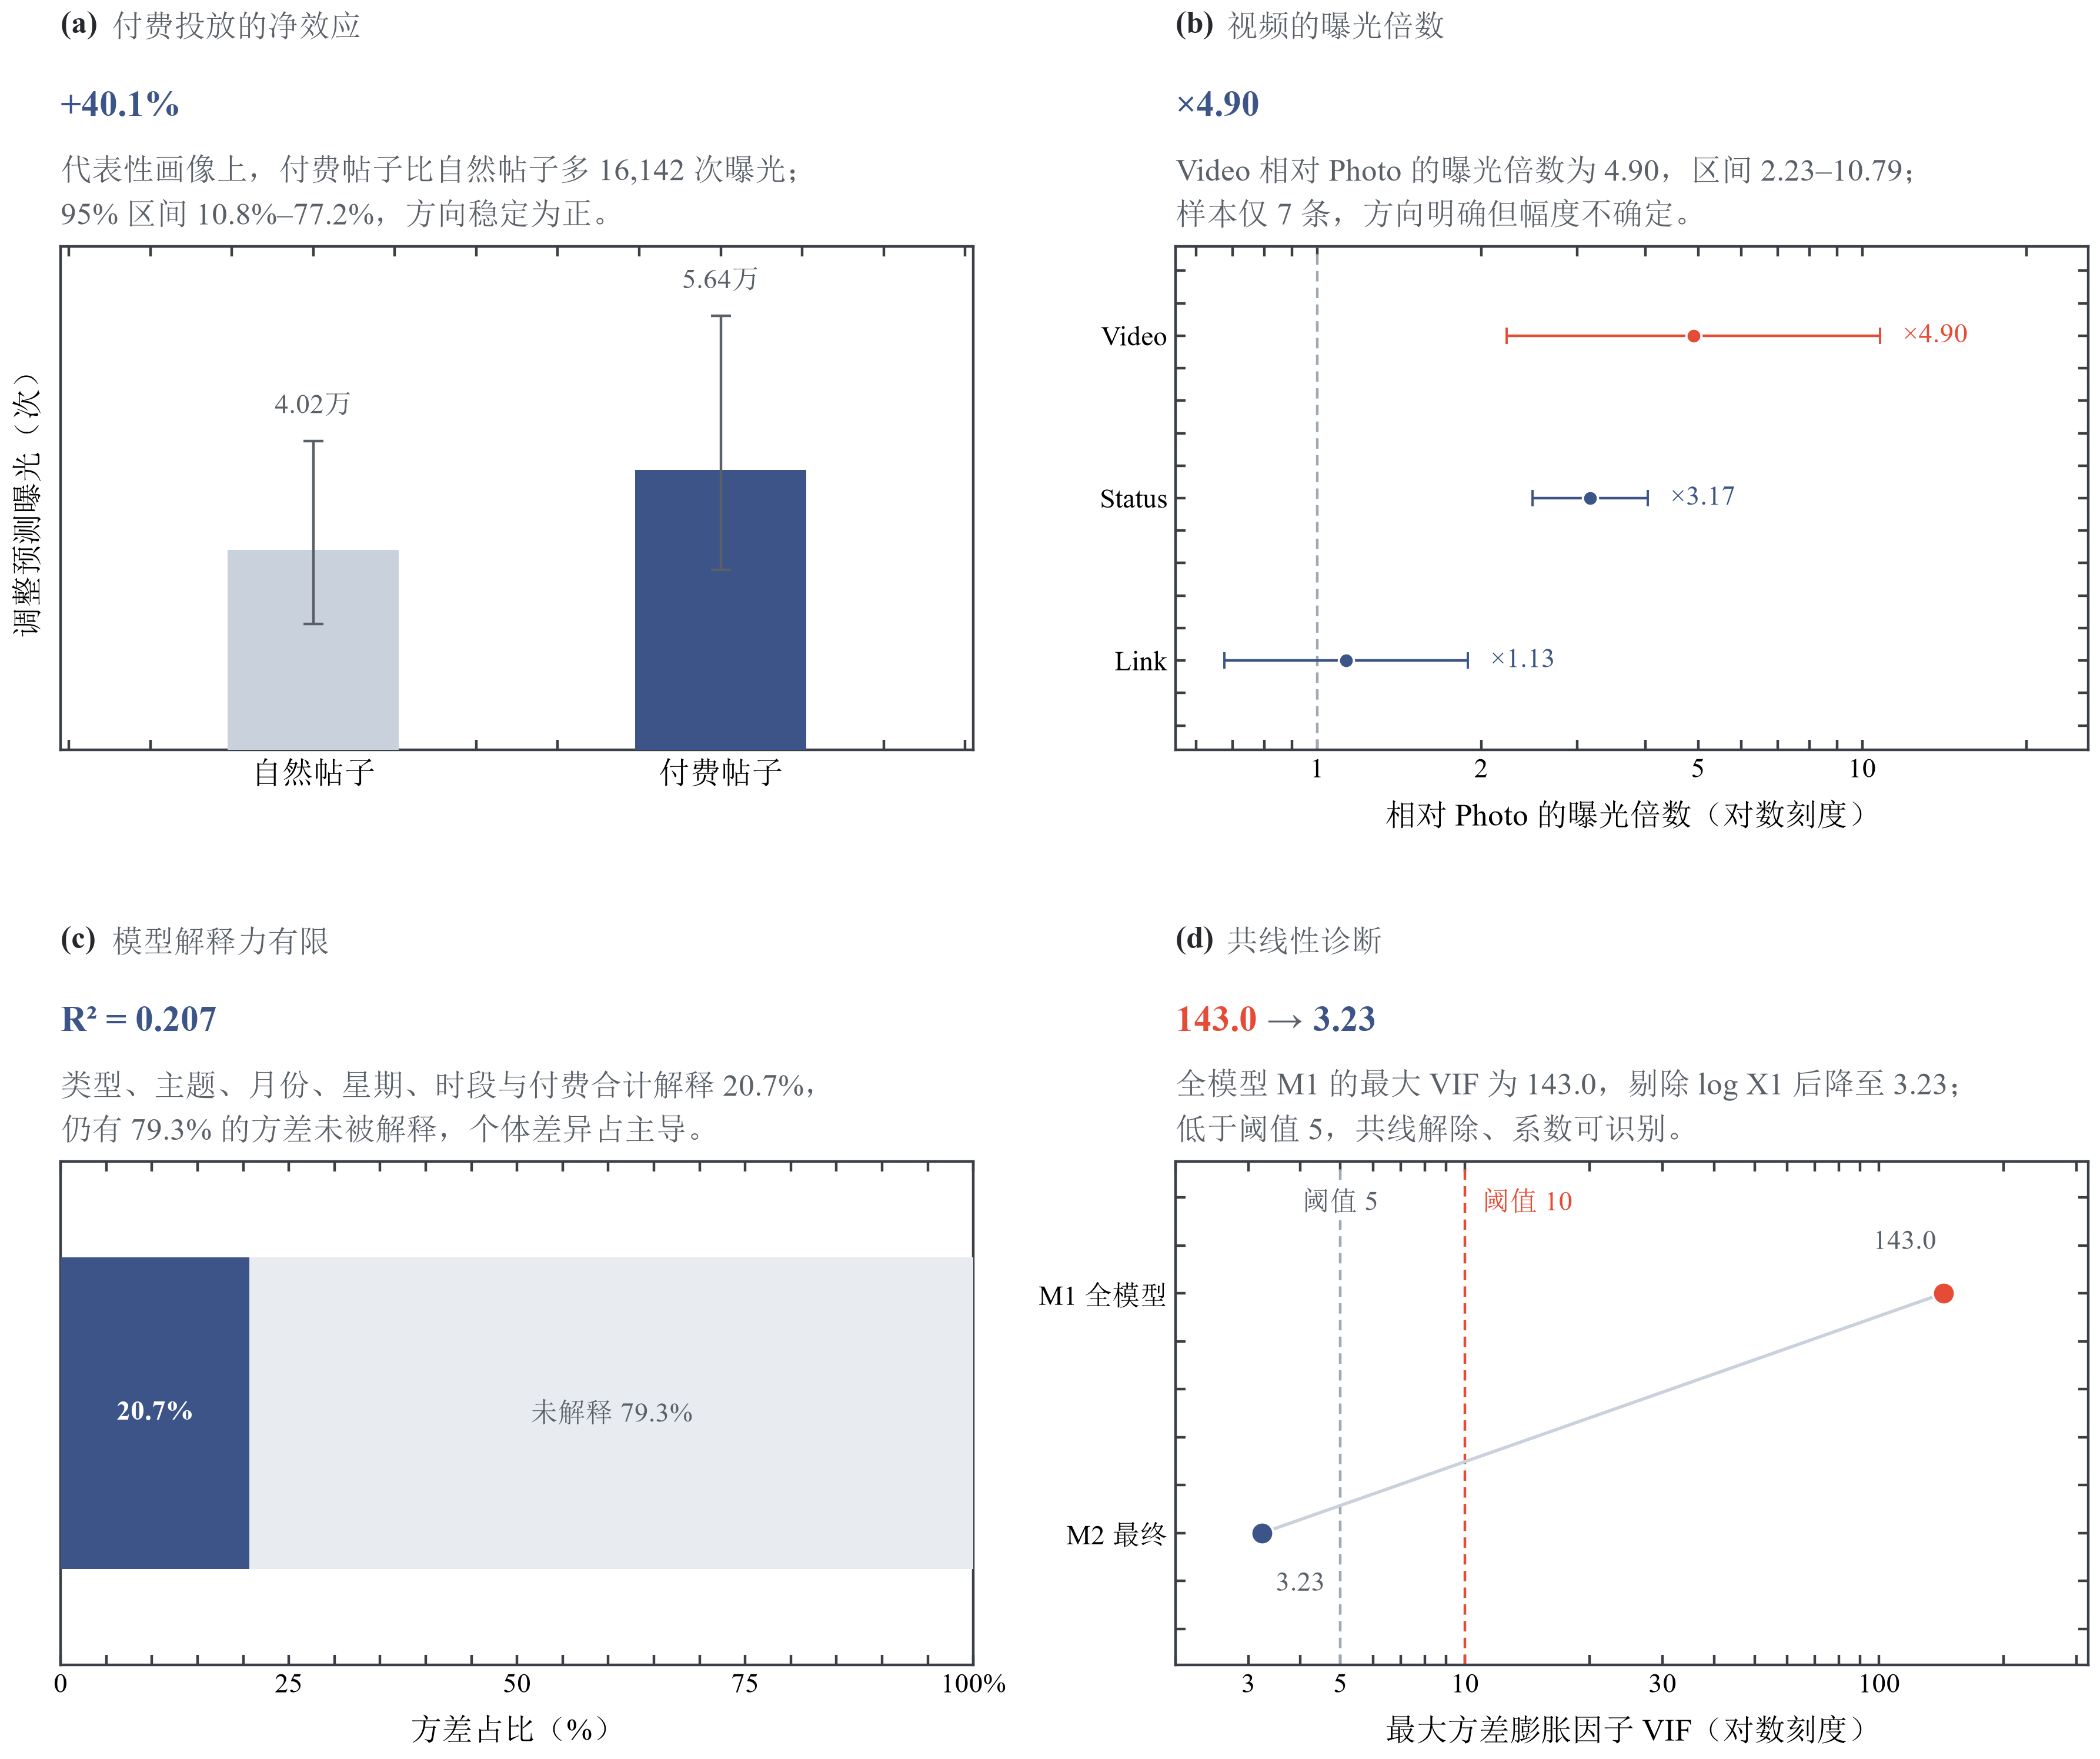
\includegraphics[width=0.76\textwidth]{../求解/临时产物/图13_核心结论总览.png}
  \caption{核心结论总览}
  \label{fig:summary}
\end{figure}

表\ref{tab:summary}把题面四项要求对应的核心估计集中列出。付费与内容类型的区间都不跨过 0（倍数不跨过 1），主题整体显著，但主题 2 与主题 3 的差异不显著；付费效应还存在主题异质性，主题 1 的增量最大，主题 3 接近于零。

\begin{longtable}{>{\centering\arraybackslash}p{0.24\textwidth}>{\centering\arraybackslash}p{0.16\textwidth}>{\centering\arraybackslash}p{0.18\textwidth}>{\centering\arraybackslash}p{0.10\textwidth}>{\centering\arraybackslash}p{0.16\textwidth}}
  \caption{核心效应汇总}
  \label{tab:summary} \\
  \toprule
  问题或效应 & 估计 & 95\% 置信区间 & $p$ 值 & 结论 \\
  \midrule
  \endfirsthead
  \caption{核心效应汇总（续）} \\
  \toprule
  问题或效应 & 估计 & 95\% 置信区间 & $p$ 值 & 结论 \\
  \midrule
  \endhead
  \bottomrule
  \endfoot
  付费平均提升 & 40.13\% & 10.80\%--77.24\% & 0.005 & 显著为正 \\
  付费画像增量 & 16,142 次 & 4,543--33,467 & — & 4.02 万$\to$5.64 万 \\
  付费全样本 ATE & 10,907 次 & 3,138--20,195 & — & 平均每条帖子 \\
  Video 对 Photo & 4.90 倍 & 2.23--10.79 & $<$0.001 & 方向明确、幅度不确定 \\
  Status 对 Photo & 3.17 倍 & 2.49--4.04 & $<$0.001 & 显著为正 \\
  Link 对 Photo & 1.13 倍 & 0.68--1.89 & 0.643 & 不显著 \\
  主题整体 & — & — & 0.0018 & 显著 \\
  主题 2 对主题 1 & 0.620 倍 & 0.475--0.808 & $<$0.001 & 显著为负 \\
  主题 3 对主题 1 & 0.730 倍 & 0.561--0.950 & 0.019 & 显著为负 \\
  主题 2 对主题 3 & 0.849 倍 & 0.666--1.082 & 0.186 & 不显著 \\
  付费 $\times$ 主题 & 组内 $P=0.036$ & — & 0.036 & 主题 1 为 0.57；主题 3 为 0.02 \\
\end{longtable}

第一，粉丝规模与月份高度共线，不能同时识别。粉丝规模与月份的 Pearson 相关系数为 0.941、Spearman 相关系数为 0.996，月份哑变量对粉丝规模对数的解释度达 99.17\%，月内方差仅占 0.83\%。这意味着粉丝规模在本样本中更接近“时间标签”而非独立解释变量，最终模型用月份固定效应吸收规模趋势，把粉丝规模留作稳健性对照，避免了把不可识别的系数当作因果效应。

第二，曝光量重尾，log1p 变换与 HC3 稳健标准误是必要处理。原始曝光量的偏度为 8.33、峰度为 93.05，变换后分别降至 0.73 与 0.82，分布接近对称；残差仍存在异方差且偏离正态，Jarque--Bera 检验拒绝正态假定，Breusch--Pagan 与 White 检验拒绝同方差假定，因此全部推断使用 HC3 标准误，使区间估计在重尾条件下仍然可靠。

第三，付费投放的平均净效应约为 40\%。最终模型的付费系数为 0.3374，折算净提升 40.13\%，95\% 置信区间为 10.80\% 至 77.24\%；代表性画像的调整预测曝光由 40,221 次升至 56,364 次，全样本平均处理效应为 10,907 次。六种模型设定下付费提升介于 37.44\% 至 49.65\%，方向一致且全部显著。

第四，内容类型差异显著，内容主题整体显著但两两差异有限。视频相对图片为 4.90 倍，置信区间 2.23 至 10.79，但视频只有 7 条样本，方向明确而幅度不确定；状态类型为 3.17 倍，链接类型为 1.13 倍且与图片无显著差异。主题 2 与主题 3 分别为主题 1 的 0.620 倍与 0.730 倍，二者都显著低于主题 1，但主题 2 与主题 3 的差异 $p$ 值为 0.186，在 5\% 水平不显著。

第五，付费效应存在主题异质性。主题组的交互联合检验 $P=0.036$，主题 1 的付费系数为 0.57（$p=0.008$），主题 2 为 0.43（$p=0.056$），主题 3 仅为 0.02（$p=0.911$）；类型组与时段组的组内 $P$ 分别为 0.531 与 0.474。付费增量主要集中在主题 1，主题 3 几乎看不到付费效果，这一发现比“平均提升 40\%”更接近可执行的投放规则。若改用互斥子样本的系数 $Q$ 检验，主题组 $p$ 值为 0.172，说明该结论对检验口径有一定敏感性，宜作为定向投放的参考而非强因果判断。

第六，发帖决策解释 14.45\% 的曝光方差，账号规模与时间解释 6.24\%，未解释部分占 79.31\%。发帖决策的贡献约为规模与时间的两倍，说明可操控的内容形式、主题与投放选择比账号自然增长更能解释帖子间的曝光差异；但两者合计仍不足总方差的三分之一，绝大多数变异来自推荐算法、受众匹配与传播随机性。

\subsection{运营建议}

对预算分配而言，付费投放应作为可控的增量工具，而不是曝光的唯一来源。40\% 是控制内容类型、主题与发布时机后的平均效应，尚未扣除投放成本；实际决策还需结合获客成本、转化率与投放目标，按边际收益而非单纯曝光增量分配预算。主题异质性提示预算不应平均撒向三类主题，而应优先投向主题 1 中已验证有效的帖子类型与时段。

对内容编排而言，视频值得小规模测试，但不宜据此制定高额投放承诺。视频的点估计最高，区间也最宽，适合以低成本试错的方式验证其在特定受众中的表现；状态类型的结果相对稳定，可作为常规内容形式；链接类型与图片无显著差异，不宜指望链接本身带来额外曝光。

对主题选择而言，应以主题 1 为基准，谨慎区分主题 2 与主题 3。两者都低于主题 1，但彼此差异不显著，过度细分主题的收益缺乏统计支持；更稳妥的做法是保持主题 1 的占比，结合受众匹配与历史互动数据做小范围 A/B 测试。付费投放应优先选择主题 1 的内容，主题 3 的付费帖在样本中几乎没有额外曝光，继续加投的性价比最低。

对预期管理而言，应把模型定位为平均效应解释工具，而不是单条帖子的曝光预测器。模型只解释约 20.7\% 的样本内方差，交叉验证拟合优度约 0.101，单条帖子的曝光受推荐机制与随机传播影响很大；用模型比较不同内容策略的平均差异是合适的，用模型承诺某条帖子的具体曝光量则不可靠。

对品牌建设而言，曝光是品牌认知的上游指标。控制其他变量后，付费帖的平均曝光约为自然帖的 1.40 倍，说明付费可放大单帖触达，但曝光只代表分发机会，不等同于品牌记忆或好感。主题 1 的稳定优势说明其更契合当前受众偏好，可作为品牌内容主线；主题 2 与主题 3 的差异不显著，则提示细分主题尚未形成清晰定位。视频波动大，适合作为品牌内容的试验田，不宜作为主渠道。数据缺少互动与转化指标，本报告只能判断曝光层面的品牌触达，品牌资产的长期变化仍需另行评估。
